% Intended LaTeX compiler: pdflatex
\documentclass[12pt, a4paper]{memoir} 
 \usepackage[french, english]{babel}
\usepackage [vscale=0.76,includehead]{geometry}                % See geometry.pdf to learn the layout options. There are lots.
\usepackage{lipsum}
\usepackage{graphicx}
\usepackage{amsmath}
\usepackage{fullpage}
\usepackage{mathptmx} % font = times
\usepackage{helvet} % font sf = helvetica
\usepackage[utf8]{inputenc}
\usepackage{relsize}
\usepackage[T1]{fontenc}
\usepackage{tikz}
\usepackage{booktabs}
\usepackage{textcomp}%textquotesingle
\usepackage{multirow}
\usepackage{pgfplots}
\pgfplotsset{compat=1.13}
\usepackage{url}
\usepackage{footnote}
\usepackage[pdfusetitle, colorlinks=true]{hyperref} %http://www.ctan.org/tex-archive/macros/latex/contrib/hyperref/
\hypersetup{allcolors=black}
\usetikzlibrary{arrows,shapes,positioning,shadows,trees,calc}
\makesavenoteenv{tabular}
\makesavenoteenv{table}
\def\checkmark{\tikz\fill[scale=0.4](0,.35) -- (.25,0) -- (1,.7) -- (.25,.15) -- cycle;}
\usepackage{listings}
\usepackage{color}
\usepackage{xspace}
\usepackage{subcaption}
\usepackage{verbments}
\usepackage{minted}
\usepackage{enumitem}
\setitemize{noitemsep,topsep=0pt,parsep=0pt,partopsep=0pt}

  \usepackage{graphicx}
  \usepackage{hyperref}
\date{\today}
\title{}
\hypersetup{
 pdfauthor={},
 pdftitle={},
 pdfkeywords={},
 pdfsubject={},
 pdfcreator={Emacs 24.5.1 (Org mode 9.0.4)}, 
 pdflang={English}}
\begin{document}

\let\oldref=\ref
\def\ref#1{~\oldref{#1}\xspace}


\lstset{ %
  basicstyle=\footnotesize,        % the size of the fonts that are used for the code
  breakatwhitespace=false,         % sets if automatic breaks should only happen at whitespace
  breaklines=true,                 % sets automatic line breaking
  captionpos=b,                    % sets the caption-position to bottom
  %commentstyle=\color{mygreen},    % comment style
  deletekeywords={...},            % if you want to delete keywords from the given language
  escapeinside={\%*}{*)},          % if you want to add LaTeX within your code
  extendedchars=true,              % lets you use non-ASCII characters; for 8-bits encodings only, does not work with UTF-8
  frame=single,	                   % adds a frame around the code
  keepspaces=true,                 % keeps spaces in text, useful for keeping indentation of code (possibly needs columns=flexible)
  keywordstyle=\color{blue},       % keyword style
  language=C,                 % the language of the code
  otherkeywords={*,...},           % if you want to add more keywords to the set
  numbers=left,                    % where to put the line-numbers; possible values are (none, left, right)
  numbersep=5pt,                   % how far the line-numbers are from the code
  %numberstyle=\tiny\color{mygray}, % the style that is used for the line-numbers
  rulecolor=\color{black},         % if not set, the frame-color may be changed on line-breaks within not-black text (e.g. comments (green here))
  showspaces=false,                % show spaces everywhere adding particular underscores; it overrides 'showstringspaces'
  showstringspaces=false,          % underline spaces within strings only
  showtabs=false,                  % show tabs within strings adding particular underscores
  stepnumber=2,                    % the step between two line-numbers. If it's 1, each line will be numbered
  stringstyle=\color{mymauve},     % string literal style
  tabsize=2,	                   % sets default tabsize to 2 spaces
  title=\lstname                   % show the filename of files included with \lstinputlisting; also try caption instead of title
}
\renewcommand{\lstlistingname}{Code}

%Style des têtes de section, headings, chapitre
\headstyles{komalike}
\nouppercaseheads
\chapterstyle{dash}
\makeevenhead{headings}{\sffamily\thepage}{}{\sffamily\leftmark}
\makeoddhead{headings}{\sffamily\rightmark}{}{\sffamily\thepage}
%\makeoddfoot{plain}{}{}{} % Pages chapitre.
\makeheadrule{headings}{\textwidth}{\normalrulethickness}
\renewcommand{\chaptername}{\relax}
\renewcommand{\chaptitlefont}{ \sffamily\bfseries \LARGE}
\renewcommand{\chapnumfont}{ \sffamily\bfseries \LARGE}
\setsecnumdepth{subsection}


\pretitle{\HUGE\sffamily \bfseries\begin{center}}
\posttitle{\end{center}}
\preauthor{\LARGE  \sffamily \bfseries\begin{center}}
\postauthor{\par\end{center}}
\newcommand{\jury}[1]{%
\gdef\juryB{#1}}
\newcommand{\juryB}{}
\newcommand{\session}[1]{%
\gdef\sessionB{#1}}
\newcommand{\sessionB}{}
\newcommand{\option}[1]{%
\gdef\optionB{#1}}
\newcommand{\optionB}{}

\renewcommand{\maketitlehookd}{%
\vfill{}  \large\par\noindent
\begin{center}\juryB \bigskip\sessionB\end{center}
\vspace{-1.5cm}}
\renewcommand{\maketitlehooka}{%
\vspace{-1.5cm}\noindent\includegraphics[height=12ex]{pics/logo_uga.pdf}\hfill\raisebox{2ex}{\includegraphics[height=14ex]{pics/logo_inp.pdf}}\\
\bigskip
\begin{center} \large
Master of Science in Informatics at Grenoble \\
Master Informatique \\
Specialization \optionB  \end{center}\vfill}
% End of title page formatting

\option{Parallel, Distributed \& Embedded Systems}
\title{Capacity Planning of Supercomputers\\\vspace{-1ex}\rule{10ex}{0.5pt} \\Simulating MPI Applications at Scale}
\author{Tom Cornebize}
\date{21 June 2017} % Delete this line to display the current date
\jury{
Research project performed at Laboratoire d'Informatique de Grenoble\\\medskip
Under the supervision of:\\
Arnaud Legrand\\\medskip
External expert:\\
Swann Perarnau\\
Defended before a jury composed of:\\
Massih-Reza Amini\\
Sihem Amer-Yahia\\
Olivier Gruber\\
}
\session{June \hfill 2017}
\setcounter{tocdepth}{4}
\setcounter{secnumdepth}{4}

\selectlanguage{English} % french si rapport en français
\frontmatter
\begin{titlingpage}
\maketitle
\end{titlingpage}

%\small
\setlength{\parskip}{-1pt plus 1pt}

\renewcommand{\abstracttextfont}{\normalfont}
\abstractintoc
\begin{abstract}
The capacity planning of supercomputers is a complex but important task. The best combination of hardware for the given
budget has to be selected. Such choices are often guided by some common rules, elaborated after years of trial and
error. The rapid development of the field, however, makes this approach costly and ineffective. We believe that experts
could benefit from accurate and efficient simulators to design the next generations of supercomputers. In this work, we
simulate a complex MPI application at the scale of the current top500 supercomputers, using the Simgrid simulation
toolkit. We present the optimization developed to enable this kind of large scale executions, we demonstrate the
soundness of the resulting simulation and we illustrate the new possibilities of study.
\end{abstract}
\abstractintoc
\renewcommand\abstractname{Acknowledgement}
\begin{abstract}
A lot of persons have contributed to my work. I would like to warmly thank them all. In particular:
\begin{itemize}
    \item Arnaud Legrand, my supervisor, for welcoming me in his team and advising me during this internship. His
          help about a wide range of topics has been very precious.
    \item Christian Heinrich, who taught me how to use Org mode and gave me multiple advices.
    \item Martin Quinson, for reviewing my pull requests and helping me to improve them.
    \item Vincent Danjean, Augustin Degomme, and Samuel Thibault, for their technical help on various parts of the implementation.
    \item Emmanuel Agullo and Abdou Guermouche, for their advices on the simulation of HPL.
    \item All the other members of the Simgrid project, POLARIS and DATAMOVE teams, PhD students and interns, who all contributed to the good mood.
\end{itemize}
\end{abstract}
\renewcommand\abstractname{Résumé}
\begin{abstract} \selectlanguage{French}
La conception d'un supercalculateur est une tâche complexe. La meilleure combinaison de matériel pour un budget donné
doit être sélectionnée. De tels choix sont souvent guidés par des règles communes, élaborées après des années d'essai
et erreur. Le développement rapide du domaine rends cette approche couteuse et inefficace. Nous pensons que les experts
pourraient bénéficier de l'utilisation de simulateurs précis et efficaces pour concevoir les prochaines générations
de supercalculateurs. Dans ce rapport, nous simulons une application MPI complexe à l'échelle des supercalculateurs du
top500 actuel, en utilisant l'outil de simulation Simgrid. Nous présentons les optimisations développées pour permettre
ce type d'exécutions à grande échelle, nous démontrons la fiabilité de la simulation et nous illustrons les nouvelles
possibilités d'étude.
\end{abstract}
\selectlanguage{English}

\cleardoublepage

\tableofcontents* % the asterisk means that the table of contents itself isn't put into the ToC
\normalsize

\mainmatter
\SingleSpace


\chapter{Introduction}
\label{sec:orgc117885}
\subsection{High Performance Computing (HPC)}
\label{sec:org0358c93}
Nearly all scientific fields have needs for computation power. This includes simulations of the Big Bang as well as
simulations of molecules interactions or air flows against a plane wing. The performance of computers has
tremendously increased in the last decades, allowing to perform larger computations. For instance, the cost to
sequence an entire human genome has decreased from approximately \$100M in 2001 to \$1k nowadays.

This gain of performance used to be explained by Moore's law. This is an observation stating that the number of
transistors in an integrated circuit doubles approximately every two years. Because of physics constraints, it seems
not possible to improve the performance of processors by miniaturizing further their transistors or increasing their
clock speed. To keep the quest for high performance, it is necessary to build multi-cores, multi-processors and
even multi-nodes computers exploiting all kind of complex network, memory hierarchy and accelerators.

The most commonly used idiom to program supercomputers is the Message Passing Interface\footnote{\url{http://mpi-forum.org/}}. This is a standard
defining the syntax and semantics of communication primitives. Several C implementations exist, including Open
MPI\footnote{\url{https://www.open-mpi.org/}} and MPICH\footnote{\url{https://www.mpich.org/}}. Some important features of MPI are point-to-point communications, i.e., one
process sends a message to another process, and collective communications, i.e., a group of processes exchange one or
several messages in a specific way.

Designing such supercomputers and parallel applications is particularly challenging and is currently a very active
research area.
\subsection{Simulation}
\label{sec:org37962c7}
Experimentation is one of the pillars of science and the scientific method, mainly used to confirm or refute
hypothesis. Some experiments may be too long to conduct, too costly, unethical or even unfeasible. For instance, car
manufacturers try to avoid performing too much crash tests. It is also not possible to create a black hole in a
laboratory. In such cases, doing a simulation may be a better or even the only way.

For the same reason, simulation is often used in computer science and in particular in HPC research. There exists
simulators of peer to peer network as well as simulators of micro-architecture. Simgrid\footnote{\url{http://simgrid.gforge.inria.fr/}} is a project
that aims at sound and efficient simulations of various distributed systems. It can be used, among other
functionalities, to simulate MPI applications.
\subsection{Contribution}
\label{sec:orgb2f02f5}
The main contribution of this work is the simulation of the High Performance LINPACK (HPL) benchmark at large
scales with Simgrid. HPL is a dense linear algebra benchmark, based on MPI, widely used in the HPC community in
particular to compare the performance of supercomputers. While it is possible to effortlessly simulate the execution
of HPL with Simgrid, doing so efficiently is far from trivial. We present in this report the different optimizations
we had to develop, both for HPL and Simgrid itself, to enable the simulation of executions several orders of
magnitude larger than what can be traditionally achieved. Our optimizations allow us to simulate configurations
similar to the ones encountered on real supercomputers.
\subsection{Outline}
\label{sec:org0dff904}
The context of this work is presented in chapter \ref{sec:org16f33bb}. In chapter \ref{sec:orgf52ffec}, the state of the art
techniques for the simulation of MPI applications are presented, as well as the main simulators in the context of
MPI application simulation. The main contribution consists in chapter \ref{sec:org5bef26f}, where the different
optimizations we implemented are explained and evaluated. Finally, chapter \ref{sec:org1697fb2} validates
experimentally the soundness of the simulation and shows the type of studies that are now feasible thanks to the
increased efficiency.
\chapter{Context}
\label{sec:org16f33bb}
The HPC community has been very active in the last 40 years. In the 1980s, the supercomputers were made of a few
powerful nodes. There also was some attempts with large numbers of lightweight nodes. Later, in the 1990s, when
personal computers began to be widespread, people started to use commodity clusters for HPC. The 2000s saw the
appearance of multi-core processors. Finally, since the beginning of the 2010s, an increasing number of supercomputers
use hardware accelerators, such as GPU or Intel's Xeon Phi. All these configurations have multiple computing units
that need to be efficiently interconnected.
\section{HPC topology and performance}
\label{sec:org320d296}
\subsection{HPC topology}
\label{sec:org45ac58b}
The choice of the topology for a supercomputer is critical. It should have good performance while remaining at a
(relatively) low cost. A network unable to handle the communication workload will slow down significantly the
applications, but also cause a low energy efficiency due to the important consumption of idling CPUs for little
benefit. A good topology should have:
\begin{itemize}
\item Short routes between nodes. The shorter they are, the lower is the latency.
\item A large bisection bandwidth. This measures the bandwidth between two arbitrary halves of the topology. It is
particularly useful for large jobs.
\item A good separability. Independent jobs can be scheduled in different parts of the topology that have a low
interference for each other.
\end{itemize}

A very popular topology in current HPC platforms is the fat tree\cite{Zahavi10}. Figure~\ref{fig:fat_tree} is an
example of fat tree with three levels. The circles represent switches, the squares compute nodes. The intuition
behind this topology is that a tree should have “fatter” links near the root than near the leaves, to preserve the
overall bandwidth. More precisely, on a tree where switches have K down ports and one up port, the up port should
have a capacity K times higher than each of its down ports. In practice, this is unfeasible, all links have the same
capacity. Thus, multi-rooted “trees” are used: every switch has several down ports and up ports. Fat tree topologies
are said to be non-blocking, meaning that there always exists independent paths between all pairs of nodes in the
system, thus enabling simultaneous communications without contention. In practice\cite{conf/cluster/DesaiBSI08},
\emph{pruning} is often done on fat trees. This consists in removing some links and switches in the upper layers of the
tree. It has been shown\cite{Leon:2016:CPS:3014904.3015009} that this practice does not significantly degrade the performance of the system. The main
motivation is to reduce the cost of the network or even its energy consumption.

A fat tree is uniquely described by the notation \((h ; d_1,\dots,d_h ; u_1,\dots,u_h ; p_1,\dots,p_h)\), where \(h\) is the number
of levels, \(d_i\) the number of down ports of the switches of level \(i\), \(u_i\) the number of up ports of vertices of
level \(i-1\) (including the compute nodes at level \(0\), which in practice always have one up port) and \(p_i\) is the
number of parallel ports between switches of levels \(i-1\) and \(i\).

\tikzstyle{switch}=[draw, circle, minimum width=1cm, minimum height = 1cm]
\tikzstyle{compute}=[draw, rectangle, minimum width=0.5cm, minimum height = 0.5cm, node distance=0.5cm]
\tikzstyle{base}=[ellipse, minimum width=2cm, minimum height = 0.5cm, node distance = 0.5cm]
\tikzstyle{bigswitch}=[base, draw]
\begin{figure}[htbp]
  \centering
    \begin{tikzpicture}[scale=0.4,transform shape]
	\pgfmathtruncatemacro{\size}{4}    % Number of ports in a switch, THE PARAMETER TO CHANGE
	\pgfmathtruncatemacro{\sizesquare}{\size*\size}
	\pgfmathtruncatemacro{\boundSwitch}{\size-1}
	\pgfmathtruncatemacro{\boundCompute}{\size*\size-1}
	% Compute nodes
	\foreach \i in {0,...,\boundSwitch}{
	    \pgfmathtruncatemacro{\incr}{\sizesquare*\i}
	    \foreach \x in {0,...,\boundCompute} {
		\pgfmathtruncatemacro{\z}{\x+\incr}
		\pgfmathsetmacro{\pos}{\z/2}
		\node[compute] (c_\z) at (\pos, 0) {} ;
	    }
	}
	% Switches L1 and L2
	\foreach \i in {0,...,\boundSwitch}{
	    \pgfmathtruncatemacro{\incr}{\size*\i}
	    \foreach \x in {0,...,\boundSwitch} {
		\pgfmathtruncatemacro{\z}{\x+\incr}
		\pgfmathsetmacro{\pos}{\incr*\size/2+\x*\size/2+(\boundSwitch/4)}
		\node[switch] (l1_\z) at (\pos, 4) {} ;
		\node[switch] (l2_\z) at (\pos, 8) {} ;
	    }
	}
	% Edges of the islets
	\foreach \i in {0,...,\boundSwitch}{
	    \pgfmathtruncatemacro{\incr}{\size*\i}
	    \foreach \switch in {0,...,\boundSwitch} {
		\pgfmathtruncatemacro{\sw}{\switch+\incr}
		\foreach \y in {0,...,\boundSwitch} {
		    \pgfmathtruncatemacro{\comp}{\switch*\size+\y+\incr*\size}
		    \draw (l1_\sw.south) -- (c_\comp.north);
		}
		\foreach \root in {0,...,\boundSwitch} {
		    \pgfmathtruncatemacro{\ro}{\root+\incr}
		    \draw (l1_\sw.north) -- (l2_\ro.south);
		}
	    }
	}
	\node (l1) at (-1, 4) {\Huge $L_1$} ;
	\node (l2) at (-1, 8) {\Huge $L_2$} ;
	\node (l3) at (-1, 12) {\Huge $L_3$} ;

	\pgfmathtruncatemacro{\boundDoubleSwitch}{\size*2-1}
	% Switches L3
	\foreach \x in {0,...,\boundDoubleSwitch} {
	    \pgfmathsetmacro{\pos}{\x*\size+(\boundSwitch/2)}
	    \node[switch] (l3_\x) at (\pos, 12) {} ;
	}
	% Upper edges
	\foreach \root in {0,...,\boundDoubleSwitch} {
	    \foreach \switch in {0,...,\boundCompute} {
		\pgfmathtruncatemacro{\switchmod}{mod(\switch,\size)}
		\pgfmathtruncatemacro{\rootmod}{mod(\root,\size)}
		\ifthenelse{\equal{\switchmod}{\rootmod}}{
		    \draw (l2_\switch.north) -- (l3_\root.south);
		}{}
	    }
	}
    \end{tikzpicture}
  \caption{\label{fig:fat_tree}The fat tree (3 ; 4,4,4 ; 1,4,2 ; 1,1,1)}
\end{figure}

Fat trees remain expensive, even with pruning. This motivates the development of new topologies, such as the
dragonfly\cite{Kim:2008:THD:1381306.1382129} and the hyperX\cite{Ahn:2009:HTR:1654059.1654101}. Finding out which
topology is better suited for a given application workload is an actively investigated research question.

In the next sections, we present two recent works, presented at the ACM/IEEE Supercomputing Conference of 2016. They
are representative of the kind of challenges to address when designing such interconnect.

\subsection{Topology performance}
\label{sec:org848cf2d}
Chen et all.\cite{Chen:2016:ENA:3019057.3019059} evaluated the performance of various topologies with different
workloads and routing algorithms. This is an empirical study, using a simulator.
They focus on topologies having a full uniform bandwidth, a good partitionability, which can be grown modularly and
come at a lower cost than a 3-level fat tree.


Their first test is an adversarial traffic, where task \(i\) sends to task \((i+D) \mod G\), where \(i\) and \(G\) are tuned
to be a worst case. In this case, the fat tree has great performance, regardless of the routing algorithms. Other
topologies (Dragonfly+, Stacked all-to-all, Stacked 2D hyperX) have terrible performance with direct routing. For
indirect or adaptive routing, performance is much better (but still a factor 2 lower than the fat tree).

Then, they test neighbor traffic with ideal mapping of the processes to the nodes, where the logical topology is a
grid. Again, the fat tree has nearly full performance, regardless of the routing algorithm. Other topologies have
lower performance with indirect routing, but good enough with direct or adaptive routing.

The authors then had a look at random-mappings of the processes to the nodes. This could reflect what would do a
scheduler which is not topology-aware.  In general, with adaptive routing, the Fat Tree and the Dragonfly+ are very
robust to irregular placements, the completion time is not impacted too much. This is not the case for stacked
topologies (due to a lack of path diversity). Thus, we should use a topology-aware job scheduler, especially for
stacked topologies.  With non-adaptive routing, all the topologies suffer of performance degradation.
\subsection{Applications performance}
\label{sec:orgfb9773e}
León et al.\cite{Leon:2016:CPS:3014904.3015009} characterized the behavior of applications that run on
their fat tree cluster, with an emphasis on communication requirements. The main motivation is to make more informed
choices when building new clusters (should we use our budget to get more links or more nodes?).  Measurements on the
cluster over one week show that the network is not used very much: the maximal link utilization is approximately
50\%, the average link utilization is 2.4\%. Doing the same measures with a tapered fat tree (one of the two root
switches is turned off) shows a very low impact on link utilization, except for some outliers.

Then, the authors recorded which type of jobs were submitted. A great majority of them was really small.  95\% of
jobs have at most 16 nodes, 76\% have only one node. Moreover, jobs of less than 64 nodes consume 75\% of the time.
Thus, if the jobs are well-placed, the need for distant communications is very low, which explains the good
performance of the tapered fat tree. This shows that a good understanding of the intended utilization of a cluster
is key.

The authors also conducted some experiments on the tapered fat tree, both with real executions and simulations, with
different number of nodes. They tested “real life” applications having very different behaviors: different
communication to computation ratio, different use of collective communication. They found that the impact on
performance was negligible for most of them, the highest slow-down being 2\%.

\section{Top500 and the HPL benchmark}
\label{sec:orgb455b0c}
The top500 list\footnote{\url{https://www.top500.org}} is a ranking of the 500 most powerful supercomputers in the world, proposed by Jack
Dongarra in 1993 and updated every year since then.  This ranking is established by running the High Performance
LINPACK (HPL) benchmark\cite{Dongarra03thelinpack} on the supercomputers. It is a C program that evaluates the
performance of a parallel computer, in terms of floating-point operations per second (flops). To do so, it computes
the LU factorization of a matrix \(A \in \mathbf{R}^{n \times n}\) in 64-bit floating-point arithmetic and reports the
duration. Such factorization requires a number \(\mathrm{flop}(n)\) of floating-point operations equal to:
\[\mathrm{flop}(n) = \frac{2}{3}n^3 + 2n^2 + O(n)\]

The LU factorization can then be used to efficiently solve a matrix equation of order \(n\):
\[Ax = b ; A \in \mathbf{R}^{n \times n} ; x,b \in \mathbf{R}^n\]

HPL takes as input, among other arguments, the size of the matrix and the number of processes. It outputs the
duration of the resolution and the estimated performance, in Gflops. This performance is equal to
\(\mathrm{flop}(N)/\mathrm{time}\).

The implementation of this benchmark is based on an implementation of MPI for the communications and an
implementation of the Basic Linear Algebra Subprogram (BLAS) for the computations. Such a factorization works with
blocks of size \(B\) and is made of \(n/B\) steps corresponding to an outer loop with an index \(k\) ranging from \(n/B\) to
\(1\). At each step, the algorithm processes a sub-matrix of size \((n-kB)\times(n-kB)\) well-balanced between all the
processes and calls the BLAS kernels. Although the communication patterns at each step essentially consists of reduce
and broadcast operations, HPL does not rely on the default MPI collective operations, which are blocking. Instead, to
ensure a good overlap of communications with computations, it provides its own custom implementation of the
collective communications.

To illustrate the size of the larger supercomputers, the machine currently occupying the first place in the top500 is
Sunway TaihuLight, located in the National Supercomputing Center in Wuxi (China). It is made of 40,960 nodes
comprising a total of 10,649,600 cores. Although this machine is relatively flat, similarly to IBM Blue Genes, many
of the other faster supercomputers comprise accelerators (GPUs or Intel Xeon Phi). This is for example the case of
Stampede, located in the Texas Advanced Computing Center (United States), and which is currently ranked \(17^{th}\) (it
was ranked \(6^{th}\) in 2013). It is made of 6400 Sandy Bridge nodes including two 8-core Xeon E5-2680 and one Intel Xeon
Phi KNC MIC coprocessor. The nodes are interconnected through a 56GB/s InfiniBand fat-tree topology.  The Stampede
supercomputer reached a performance of 5,168 Tflops to get its rank in the top500. This execution was done using \(77
   \times 78 = 6,006\) processes and a matrix of size \(n=3,875,000\). The matrix itself represents approximately 120 TB of
memory. This execution took approximately two hours.
\chapter{State of the art}
\label{sec:orgf52ffec}
The question of reproducible research is complicated in the context of distributed systems design. For instance, to
evaluate the performance of a new algorithm, one could run an experiment on some supercomputer, but this experiment
would hardly be reproducible, since not everyone would have access to the same machine. To overcome this, a lot of
research papers are based on simulation, especially recently when it comes to study the influence of various
topologies. This raises a new issue: a large number are made with one-shot programs with poor documentation, making
many simplifying assumptions. Worse, these programs are sometimes not public. It is therefore important to have
simulators whose soundness has been rigorously established and which are publicly available to the whole community.

There are several typical use cases motivating the simulation of supercomputers:
\begin{itemize}
\item Sensibility analysis and capacity planning, which aims at understanding the influence of key parameters. \emph{What will
be the performance if we take a larger version of our hardware?} \emph{What will be the performance if we take different
hardware?}
\item Detection of hardware misconfiguration, leading to unexpected performance behaviors.
\item MPI runtime and application tuning, for instance choosing the algorithms of MPI collective operations.
\item Teaching, supercomputers are expensive infrastructures, we cannot let the students play with them.
\end{itemize}

The goal of this section is to present the various possible approaches in term of simulation of HPC
infrastructures. This presentation mostly builds on \cite{casanova:hal-01017319,degomme:hal-01415484,legrand:tel-01247932} written by the
Simgrid team. In section \ref{sec:org27c0a2f} we review the different approaches and trade-offs to consider. We then present
the main simulation projects existing in this context in section \ref{sec:orgbd107bb}. Finally, we give an overview of SMPI
in section \ref{sec:orgc53d7b7}, a simulator of MPI applications building on the Simgrid framework and which we used to simulate
HPL at scale.
\section{Features of a simulator}
\label{sec:org27c0a2f}
\subsubsection{Capturing the behavior of an application.}
\label{sec:orgda424dc}
Two main approaches exist to capture the behavior of an application, \emph{off-line} simulation and \emph{on-line} simulation.

With off-line simulation, a trace of MPI communication events is first obtained by running the application. The
durations of the CPU bursts are measured during the trace generation. Then, when replaying the trace of the
application on top of the simulator, they are modified to account for the performance differences between the
target platform and the platform used to obtain the traces. This approach is relatively fast and simple to
implement but suffers from at least three limitations. First, the acquisition of the trace requires to perform a
real execution. This may be problematic if one wants to simulate a large platform but has none at disposal. Second,
the resulting trace can become very large, in the order of hundreds of gigabytes. The processing of such traces can
take a significant amount of time. A solution is to record only aggregated statistics, which may be enough to
detect some anomalies, but prevent a more in-depth analysis. Third, extrapolation may be difficult. In particular,
off-line simulation does not make sense for applications that adapt their behavior to the platform or the input.

With on-line simulation, the actual application code is executed, part of the instruction stream is intercepted and
passed to a simulator (typically, the communication primitives). It is thus a form of “emulation”, in the sense
that the application is executed in a virtualized environment. It may be ran on a simple laptop but behaves as if
it was executed on a supercomputer. There are several possibilities to capture MPI calls. One is to use PMPI
interface (provided by every MPI implementation), which allows to attach callbacks to every MPI functions. However,
for collective operations, this approach only captures the high-level calls, not the resulting point-to-point
communications. These collective operations therefore have to be correctly modeled, which may be difficult. Another
approach is to develop a specific MPICH or OpenMPI driver, but it ties the simulator to a specific
implementation. Finally, one can also develop an ad hoc implementation of the MPI standard.

Many applications are adaptive, even simple ones like HPL. As mentioned in section \ref{sec:orgb455b0c}, HPL
reimplements collective operations so that communications can be overlapped with computations. To this end, HPL
relies on the \texttt{MPI\_Iprobe} function. It is a non-blocking test for a message. In HPL, processes call this function at
each iteration until it returns \emph{true}. This results in a highly variable number of short messages at each
iteration. Only an on-line simulation can capture such behaviors, since the communications are fixed in an off-line
simulation.

Technically speaking, online simulation raises at least two challenges. First, a lot of MPI applications use global
variables in some places. These variables are, of course, not shared by two different MPI processes. When doing
on-line simulation however, the MPI processes are often instantiated as different threads of a same process. In
this case, the “private variable” of a MPI process becomes visible and even modifiable by other MPI processes. To
fix this, the simulator somehow needs to make sure that these variables remain private. Different approaches exist,
including source-to-source transformation, copy of the \texttt{.bss} and \texttt{.data} segments into some private zone at each
context switch or remapping of these segments. Second, the scalability of the simulation may be problematic, as
large executions may require thousands to millions of threads.
\subsubsection{Modeling the network}
\label{sec:org4b70e40}
Modeling correctly the network is one of the most important aspects in simulators. Several techniques exist.

In \emph{packet-level} simulation, the transfer of every individual packets is modeled at the level of the protocol stack. As expected, this is very
costly to simulate, so this approach is impractical at the scale we envision. It is very precise, but the model has to be very carefully
instantiated, as being precise with a wrong model is useless. Such careful instantiation can be extremely
challenging as it requires to obtain faithful information on all the different protocols of the network stack, the
characteristic of every network resource and the exact behavior of every application.

With a \emph{flow model}, the finest grain is the communication. The time to transfer a message of size S from i to j is
modeled as \(L_{i,j} + S \times B_{i,j}\).  The \(B_{i,j}\) are not constant, they need to be re-evaluated at each step of the
simulation to account for the contention of the network. This model can catch some complex behaviors, such
as RTT unfairness of TCP. The downside is that it is quite complex to implement and more costly than the delay
model.

With a \emph{delay model}, the communication times are described with some equations. One of the simplest and most popular
models in the HPC context is LogP\cite{Culler_1993}. Here, sending \(m\) bytes with packets of size \(w\) takes a time
\(2o + L + \left\lceil\frac{m}{w}\right\rceil\max(o, g)\), where \(L\) is the network latency, \(o\) the middleware
overhead, \(g\) the gap between two packets and \(P\) the number of processors. Delay models are cheap in terms of
simulations, but very imprecise. They do not take into account network topology and eventual contentions, and
suppose a processor can only send one message at a time (single-port model).
\subsubsection{Modeling the CPU}
\label{sec:org7381750}
Similarly to the network components, one can distinguish between several approaches to model the CPU.

\emph{Microscopic} models, in which every component of the CPU is accurately modeled and every instruction of the programs
is simulated at the level of CPU cycles, are very precise. However, they are also very costly and incredibly
difficult to instantiate. This approach is therefore limited to only a few nodes.

Other models have a coarser grain. For instance, the CPU load induced by communications is often neglected,
focusing on the block of codes executed between two communications, called \emph{Sequential Execution Blocks} (SEB).

A simple model is to consider that a given processor is \(x\) times faster or slower that some other
processor. Here, the simulator simply has to speed up or slow down the measured duration of the SEBs. This yields
reasonably good results for similar architectures, but this has a poor accuracy when the architectures are too
different (e.g., not only in speed, but also in the number of registers, the number of floating-point units or the
cache characteristics).

More elaborated models allow to scale differently the execution time of different blocks. These different factors
are either user-provided, or automatically determined by using some underlying models. But even these models often
fail to accurately capture the complex behavior of some modern architectures, in particular the effects on cache of
a multi-core architecture.
\subsubsection{Modeling the collective operations}
\label{sec:org1430c9d}
Again, many different approaches can be found in the literature.

In the more analytic models, each collective operation has a cost equation (depending for instance on the message
size and the number of processes). The arguments in favor and against these types of models are very similar to the
network modeling, these models are very efficient, but also very imprecise, in particular with respect to
contention.

Another approach is to benchmark each collective operation on the target platform, with various parameters and
communicators.  Then, the obtained timings are injected in the simulation. The main issues are that we cannot do
performance extrapolation with this approach, and the benchmarking phase may be very long.

Some simulators statically replace every collective operation by a semantically equivalent sequence of
point-to-point communications at compile time. This does not capture the logic of selecting the right algorithm,
which often depends on the size of the messages and is therefore only known at execution time.

Finally, some simulators implement the MPI collective operations themselves. This is a very flexible solution, but
it requires an important engineering work.
\subsubsection{Efficient simulation engine}
\label{sec:org58c98bb}
Most of the simulators rely on an efficient Discrete Event Simulation (DES) kernel, often specifically optimized
for the models and workloads to process. Events correspond to some steps of the executions of MPI processes, such
as “process i has terminated receiving a message from process j”.  To simulate large-scale executions, it is
crucial to have a very efficient DES. Some projects rely on a Parallel DES (PDES), implemented with MPI and/or
multiple threads, while others have a sequential DES and focus on its optimization (e.g., by using efficient data
structures and memory accesses).
\section{Active simulation projects}
\label{sec:orgbd107bb}
\subsubsection{Dimemas}
\label{sec:orge04b727}
Dimemas\cite{dimemas} is a project from the Barcelona Supercomputing Center (BSC). It implements off-line simulations,
using a sequential DES and uses a delay model for communications. For computations, it uses a scaling model, by
specifying the factor to apply to each SEB execution time. It is a free (as in free speech, not as in free beer)
and open-source software. Dimemas is regularly used in application diagnosis of performance issues.
\subsubsection{LogGOPsim}
\label{sec:orgfcf5df0}
LogGOPsim\cite{loggopsim_10}, developed at the University of Illinois Urbana-Champaign (UIUC) and the ETH Zurich
(ETHZ), has been specifically designed for studying collective communications at very large scale. It implements
off-line simulation, using a sequential DES.  The communications times are computed with a simple delay model,
called LogGPS. For computations, it simply applies a constant factor to all execution times. It is a free and
open-source software.
\subsubsection{SST Macro}
\label{sec:orgcdb8061}
SST Macro\cite{sstmacro} is developed at the Sandia National Laboratories and implements both off-line and on-line
simulation, using a sequential DES.  Communications are modeled either at the packet level with simple models or at
the flow level. For computations, a cycle level model is used. It is a free and open-source software.
\subsubsection{BigSIM}
\label{sec:org732f814}
BigSIM\cite{bigsim_04} is developed at the UIUC by the Charm++ development team and implements off-line simulation,
using a sequential DES.  Communications times are determined with a delay model. To model computations, the factor
to apply to the execution time of each SEB can be specified by the user. Alternatively, the execution time can be
automatically computed using some analytic memory models. It is a free and open-source software.
\subsubsection{xSim}
\label{sec:orgf4acd09}
xSim\cite{xsim} is developed at the Oak Ridge National Laboratory (ORNL) and implements both off-line and on-line
simulation, using a parallel DES.  This simulator uses a delay model for communication and does emulation to
capture the CPU behavior: it executes the application code on the target platform. It is not open source.
\subsubsection{CODES}
\label{sec:org4cfdd6c}
CODES\cite{CODES} is a recent project of the Argonne National Laboratory. It does off-line simulation, using a
generic parallel DES from the Rensselaer Polytechnic Institute: ROSS.  Communications are modeled at the flit
level. This is a finer grain than the packet level, as a packet includes one or several flits. For the
computations, this simulator apply a scaling factor per SEB. It is open source but not free.
\section{Simgrid, a simulator of distributed systems}
\label{sec:orgc53d7b7}
Simgrid is a free software to simulate a wide range of distributed systems: grid, P2P, cloud, MPI applications. It is
a joint effort of CNRS, Inria and various universities. Its simulation models have been theoretically and
experimentally assessed. The work presented in this report is based on SMPI\cite{degomme:hal-01415484}, a module of
Simgrid which can realistically simulate unmodified MPI applications.
\subsubsection{Modeling the network}
\label{sec:org39d8675}
SMPI uses a hybrid network model. Point-to-point communications are divided in three modes: asynchronous, detached
and synchronous, depending on the size of the message. Each mode has different values of bandwidth and latency,
which are estimated by doing benchmarks on real systems. To model network contentions, SMPI often relies on three logical
links for any physical link: a downlink, an uplink, and a limiter link.  The bandwidth of uploads
(resp. downloads) must be lower than the capacity of uplinks (resp. downlinks). The sum of the bandwidths must be
lower than the capacity of the limiter link. Several topologies are provided, such as the torus, the fat tree and
the dragonfly. One can also use an arbitrary topology, by describing the nodes, links, switches and routes. In the
experiments we performed, we mostly used the fat tree topology.
\subsubsection{Capturing the behavior of an application.}
\label{sec:org91d9a81}
With SMPI, it is possible to do both off-line and on-line simulations. As explained, only on-line simulation is well
suited for an application like HPL, so this is what we used. SMPI is based on a reimplementation of the MPI standard,
although not all functionalities are supported yet, in particular MPI IO.

Initially, SMPI used source-to-source transformation for the privatization of global variables. This approach was
then dropped, to use a remapping of the \texttt{.bss} and \texttt{.data} segments using the \texttt{mmap} system call. The main motivation was
the robustness of the privatization, as the initial approach had several flaws.

The work presented in this report motivated the implementation of an alternative privatization technique by the
core development team. Calling \texttt{mmap} at each context switch of MPI process has shown to be expensive for large scale
executions. The new approach creates, at the beginning of the execution, one copy of the dynamic library per MPI
process. Then, it loads all the library copies using the function \texttt{dlopen}. This function returns a \emph{handle} object,
that is then switched at each context switch of MPI process, avoiding an expensive system call.
\subsubsection{Modeling the collective operations}
\label{sec:org16f1083}
The solution used by SMPI is to implement all the collective algorithms and selection logics of both OpenMPI and
MPICH, to be sure to capture correctly the behavior of the operations. As an interesting side effect, the
user can chose the selector or the algorithm for the simulation (e.g., to compare MPICH and OpenMPI). The drawback
is that it is a tedious work for the Simgrid team.
\subsubsection{Modeling the CPU and applications at scale}
\label{sec:org1d1c791}
The approach of SMPI is to run SEB on one node of the target architecture. Then, to predict performance of a
similar architecture, the time spent in each SEB is simply scaled by some constant factor, which has to be
determined by a calibration benchmark.

In SMPI, when emulating an unmodified application, the whole application runs on a single core. Any computation
that would be made in a real execution on a real supercomputer is done in the simulation, sequentially. If a real
execution takes one hour on 64 cores, the simulation should take (at least) 64 hours on one of these cores. It is
therefore easy to see that we are limited to the study of very small configurations.

Two techniques are available for the user to decrease the simulation time and the memory consumption by exploiting
the regularity of HPC applications. They require to slightly modify the simulated application.
\begin{itemize}
\item \emph{Memory folding} is used to reduce the memory consumption. The primitives\linebreak \texttt{SMPI\_SHARED\_MALLOC} and \texttt{SMPI\_SHARED\_FREE}
can replace \texttt{malloc} and \texttt{free} in the application code.  They indicate that some data structure can safely contain
undefined data without significantly impacting the behavior of the application. The corresponding regions are
then shared using the \texttt{mmap} mechanism. A detailed explanation is given in section \ref{sec:org7de7ffe}, as we had
to extend this mechanism.
\item \emph{Kernel sampling} is used to reduce the simulation time. The primitive\linebreak \texttt{SMPI\_SAMPLE\_GLOBAL} can be used to annotate
a region of code which has a constant execution time. The first calls will be executed and their duration
measured. Then, the following calls will be skipped and the average duration of the previous calls will be
injected in Simgrid. The primitive takes two arguments: the maximal number of iterations to perform, and the
variability threshold at which SMPI can stop executing the code block.
\end{itemize}
The following is a simple example which allocates a buffer, fills it with some value, then frees it. The memory
consumption of this code as well as its execution time will be very low (despite the very large size of the
buffer).

\begin{minted}[bgcolor=white,style=tango,numbers=left,numbersep=5pt]{c}
size_t size = 1000000000;
int buff = (int*) SMPI_SHARED_MALLOC(size * sizeof(int));
for(size_t i=0; i<size; i++) SMPI_SAMPLE_GLOBAL(0.25*size, 0.03) {
    buff[i] = 42;
}
SMPI_SHARED_FREE(buff);
\end{minted}

\subsubsection{Efficient simulation engine}
\label{sec:org567945a}
SMPI is based on a fluid network model where bandwidth is regularly shared between competing flows. Such mechanisms
do not offer much room to parallelism. Therefore, Simgrid team decided to keep a sequential DES but spent a lot of
efforts optimizing it so that it can very favorably compete with other approaches.
\subsubsection{Evaluation}
\label{sec:org5db818b}
Simgrid authors conducted several experiments to demonstrate both the accuracy and the scalability of the
simulator. For instance, thanks to memory folding and kernel sampling, SMPI can simulate the NAS EP
benchmark\footnote{\url{https://www.nas.nasa.gov/publications/npb.html}} with 16,384 processes in a few hundreds seconds and less than one gigabyte of
memory\cite{degomme:hal-01415484}. Other experiments comparing SMPI simulations with real MPI executions show that
the time predictions made by the simulator has an error of less than 5\% on moderate size configurations.
\chapter{Scalable HPL simulation}
\label{sec:org5bef26f}
\section{Methodology}
\label{sec:org9d35c80}
This section presents the different optimizations that have been performed, either on HPL itself or on Simgrid, to
enable the simulation of large scale executions. Every subsection details a particular set of optimizations. It gives
the rational behind the choices that have been made, explains technical details and demonstrates through
experimentation the quality of the optimization both in terms of high performance gain and low accuracy loss.

The experiments of this section have been performed on nodes of the \emph{Nova} cluster from Grid'5000\footnote{\url{https://www.grid5000.fr}}. These nodes
have 64 GB of memory and two Intel Xeon E5-2620 v4 processors, each having eight cores. They are deployed with a
Debian Stretch image (kernel 4.9).
\subsection{Reproduce this work}
\label{sec:org2efb0ca}
This work is meant to be reproduced. For this reason, a laboratory notebook has been maintained during the whole
duration of the project. It can be reached at the following address:

\url{https://github.com/Ezibenroc/simulating\_mpi\_applications\_at\_scale}

The notebook contains instructions on how to reproduce any experimental results presented here. It also contains all
the details about our methodology. In particular, for every experiment are specified the commit hashes of the
different repositories at the moment the experiment was performed, the commands used to set up and launch the
experiment and the scripts used to process the data and generate the figures.
\section{Building on application regularity: computation kernel sampling}
\label{sec:org6b54c65}
\subsection{Profiling HPL computations}
\label{sec:org09b225d}
As explained in section \ref{sec:orgc53d7b7}, it is possible to simulate the execution of HPL without modifying it. This
simulation, that we will call \emph{vanilla HPL}, is quite inefficient.

With such approach, simulating vanilla HPL with a matrix of size 20,000 and 64 MPI processes takes 550 seconds. A
total of 536 seconds (i.e., 97\%) of this time is spent in HPL and only 14 seconds (3\%) are spent in Simgrid. A
profiling of the simulation shows that a very large part of the time is spent in the function \texttt{dgemm} (more than 90\%
for the above simulation). A significant part of the time is also spent in function \texttt{dtrsm}. These functions are part
of the Basic Linear Algebra Subprograms (BLAS) library. Function \texttt{dgemm} computes the product of two matrices of
respective sizes \(m \times n\) and \(n \times k\), function \texttt{dtrsm} solves a matrix equation \(A \times X = B\) with matrices \(A\) and \(B\)
of respective sizes \(m \times m\) and \(m \times n\). We could decrease a lot the simulation time if we somehow skipped the
expensive computations done in these functions. Our first idea was to leverage the kernel sampling mechanism
mentioned in section \ref{sec:orgc53d7b7}.
\subsection{Non-solutions}
\label{sec:orgf8cefd2}
If we want to correctly model the functions \texttt{dgemm} and \texttt{dtrsm}, it is important to understand how they are called
during the execution of HPL. To this end, we traced every call to the two functions: its location (file and line),
its parameters (sizes of the matrices) but also its duration. Figure~\ref{fig:blas_duration} shows the duration of
every call during the simulation: the x axis is the index of the call and the y axis its duration.
\begin{figure}[htpb]
\centering
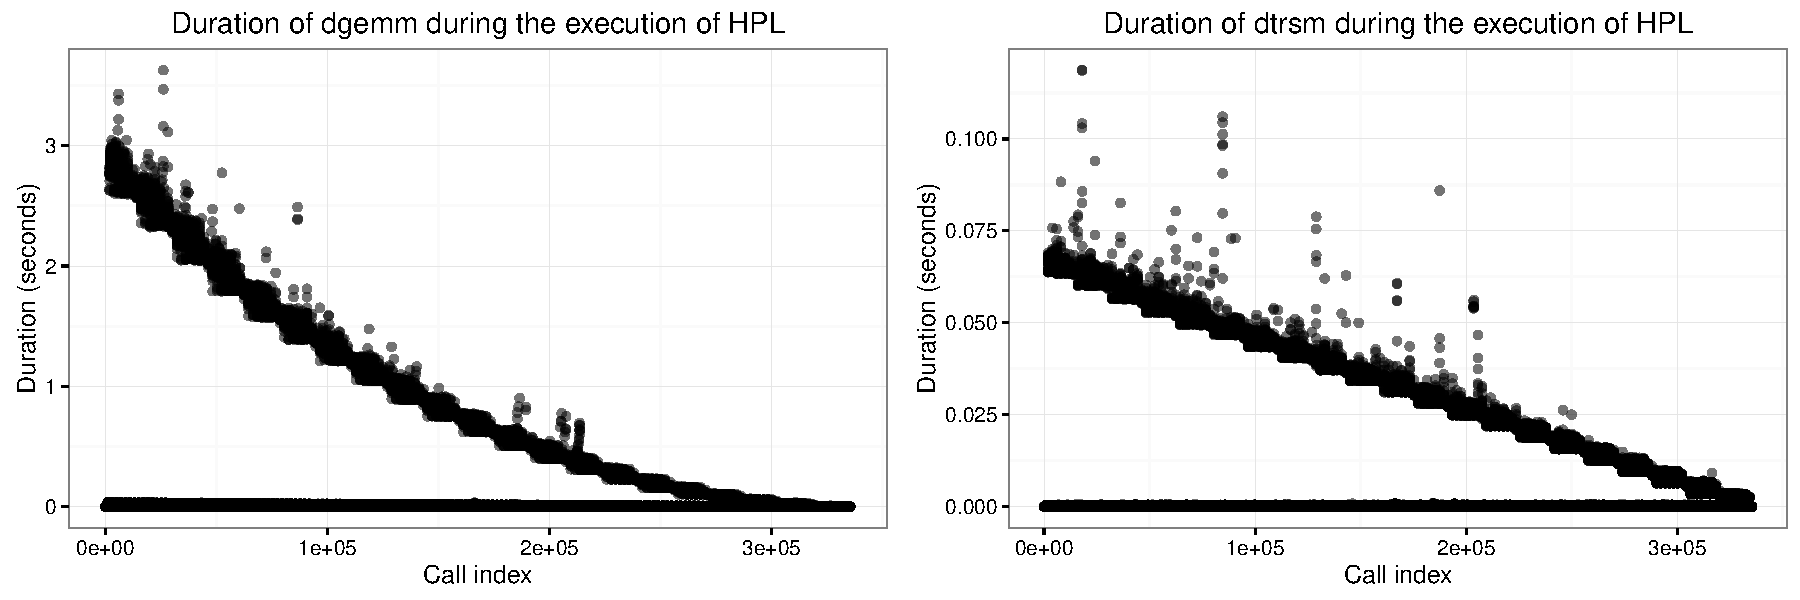
\includegraphics[width=400px]{../trace_visualization/blas_durations.png}
\caption{\label{fig:blas_duration}Duration of \texttt{dgemm} and \texttt{dtrsm} in HPL\newline64 MPI processes, matrix of size 20,000}
\end{figure}
The figure shows that, for both functions, there are two distinct and simultaneous behaviors. The first one is made
of a lot of short calls with a constant duration, the second one has calls with longer duration that decrease when
we advance in the simulation. This is due to the principle of the algorithm implemented by HPL. It does not work on
blocks with a constant size, but on the whole area at once.

This means that the simple approach previously proposed in SMPI, implemented with the macro \texttt{SMPI\_SAMPLE\_GLOBAL}, is useless
here. As explained in section \ref{sec:orgc53d7b7}, it assumes that the sampled code block has a constant execution time.

Yet, the functions \texttt{dgemm} and \texttt{dtrsm} are performing dense linear algebra operations, so their duration is very regular
and thus predictable. For instance, we can expect \texttt{dgemm} to have a complexity of \(O(m \times n \times k)\), for the
product of a \(m \times n\) matrix by a \(n \times k\) matrix. Thus, we could create a new function \texttt{SMPI\_SAMPLE\_DGEMM}
(resp. \texttt{SMPI\_SAMPLE\_DTRSM}) that works similarly to \texttt{SMPI\_SAMPLE\_GLOBAL}. First, the function executes for real the function
\texttt{dgemm} (resp. \texttt{dtrsm}) and measures its execution time. When enough data is collected, the function performs a linear
regression with the right model (e.g., \(m \times n \times k\) for \texttt{dgemm}) and injects time predictions for the following calls.

The issue with this approach is that we would still have to run some (expensive) calls, since the longest ones are
at the beginning of the execution, as shown by figure~\ref{fig:blas_duration}. This cost would not only be
prohibitive for simulations with large matrices, but this approach would also have to re-do the measurements and the
regression for every simulation, which is a waste of time.
\subsection{Off-line modeling of computation kernels}
\label{sec:org04b4653}
The solution we propose is not to do a linear regression during the simulation, or \emph{on-line}, but to do a regression
before the simulation, or \emph{off-line}, and somehow independently from HPL.

The first step is to implement a small C program for each of the two functions. These programs take as an argument
the sizes of the matrices. Then, they allocate the matrices, run the desired BLAS function while measuring its
execution time, free the matrices and finally output the time.

A Python script is used to perform the measurements and export them as a CSV file. It takes a number of experiments
to run and a maximal size. For each experiment, it chooses randomly and uniformly the sizes of the matrices between
1 and the maximal size. Then, it runs the program, gets the execution time and adds an entry in the file, with the
sizes and the time.

To find the right model for each of the functions, a first analysis is needed. Our first guess was that \texttt{dgemm} had a
complexity of \(m \times n \times k\), but this has to be checked. In particular, there could be lower order terms that are
non-negligible for the range of sizes we consider. To do so, we use the R programming language.
\begin{itemize}
\item For the \texttt{dgemm} function, we perform a first linear regression where the model is a polynomial of degree 3 in \(m, n\)
and \(k\). The regression shows that the only significant term is \(m \times n \times k\). After, we fit a second linear
regression, with \(m \times n \times k\) for model, we find a \(R^2\) of 0.9997, which is a sign of a very good fit and that
almost no variability is left unexplained.
\item For the \texttt{dtrsm} function, we also do a first regression with a polynomial of degree 3 in \(m\) and \(n\) as a model. The
regression shows that the only significant term is \(m \times n^2\). We do a second linear regression, with \(m \times n^2\) for
model. We find a \(R^2\) of 0.9994, which is again very good.
\end{itemize}
A graphical verification of the regression is shown in figure~\ref{fig:blas_regression}. The points have been obtained by
running the aforementioned script. The line has been drawn with the equation \(time = \alpha x\) where \(\alpha\) is the
coefficient found by the linear regression and \(x\) is the product of the sizes. It makes no doubt that the model is
correct and should be useful for predictions.
\begin{figure}[htpb]
\centering
\begin{subfigure}{.5\textwidth}
  \centering
  \includegraphics[width=\linewidth]{../blas_reg/dgemm.pdf}
\end{subfigure}%
\begin{subfigure}{.5\textwidth}
  \centering
  \includegraphics[width=\linewidth]{../blas_reg/dtrsm.pdf}
\end{subfigure}
\caption{Linear regression of dgemm and dtrsm}
\label{fig:blas_regression}
\end{figure}

For convenience, another Python script takes the CSV files containing the raw results of the two functions, performs
the linear regression with the right model for each function and returns the coefficient to use, thus skipping the
step of the model choice.

Now, the modification to HPL is made by defining the macro \texttt{HPL\_dgemm} as follows (the modification for \texttt{dtrsm} is similar):

\begin{minted}[bgcolor=white,style=tango,numbers=left,numbersep=5pt]{c}
#define  HPL_dgemm(layout, TransA, TransB, M, N, K, alpha, A,\
        lda, B, ldb, beta, C, ldc)  ({\
    double expected_time = ((double)(SMPI_DGEMM_COEFFICIENT))*\
        ((double)(M))*((double)(N))*((double)(K));\
    if(expected_time > 0)\
        smpi_execute_benched(expected_time);\
})
\end{minted}

The value of the variable \texttt{SMPI\_DGEMM\_COEFFICIENT} (resp. \texttt{SMPI\_DTRSM\_COEFFICIENT}) is passed at compile time. It is
determined by running the Python script on the target machine once and for all.

\subsection{Validation}
\label{sec:orgbd31c09}
The validation step is required to verify that after our modifications, the estimation is still accurate and that we
fulfilled the objective, that is decreasing the simulation time. To verify this, we compare the two versions of HPL:
the vanilla version and the “optimized” version. Comparison with real life experiments will be given in section
\ref{sec:org8c1d01f}.

Figure~\ref{fig:L1_gflops} shows the estimation of the performance of the platform, in Gflops, as returned by
HPL. The closer the two versions of HPL, the better. Here, the error made by HPL with kernel sampling is less than
10\%, in comparison with vanilla HPL. This should be good enough to observe the same trends (e.g., a drop of
performance due to network contention), but an improvement in the prediction accuracy would still be desirable.

A hypothesis for this inaccuracy is that, as shown in figure~\ref{fig:blas_duration}, there are a significant
number of outliers in the execution times of \texttt{dgemm} and \texttt{dtrsm} when running the vanilla HPL emulation. For \texttt{dgemm},
plotting this execution time against \(m \times n \times k\) (resp. \(m \times n^2\) for \texttt{dtrsm}) shows that these outliers are still
present: we are not observing “unusual” sizes in the execution of HPL, but really “unusually large” times. Since the
real times are larger than the expected times, this explains why HPL with kernel sampling appears overly optimistic
in terms of performance compared to vanilla.

The cause of these outliers is not clear, as we could not reproduce them by running the two BLAS functions outside of
HPL (see figure~\ref{fig:blas_regression}, where all the observed times are very close to the prediction of our
model). One reason could be that a long simulation has more chances to be subject to some perturbations.

\begin{figure}[htpb]
\centering
\includegraphics[width=\linewidth,page=2]{../validation/L1/report_plot_gflops.pdf}
\caption{Gflops estimation with and without kernel sampling}
\label{fig:L1_gflops}
\end{figure}

Figure~\ref{fig:L1_simulation_time} compares the simulation time of both versions of HPL. We want this time to be
the lower possible. The benefit of using kernel sampling is very clear from these plots as the new simulation times
are one order of magnitude lower.

Now, the simulation with a matrix of size 20,000 and 64 MPI processes takes a time of 44 seconds, compared to the
550 seconds for the vanilla simulation. A total of 30 seconds (i.e., 68\%) of this time is spent in HPL, the rest of
the time (still 14 seconds) is spent in Simgrid.

There is still room for optimization. First, 68\% of the time spent in the application is still too high, it should be
lower. Also, the simulation time looks to be quadratic in the matrix size, which would still prevent to do
simulations with very large sizes.

\begin{figure}[htpb]
\centering
\includegraphics[width=\linewidth,page=2]{../validation/L1/report_plot_time.pdf}
\caption{Simulation time with and without kernel sampling}
\label{fig:L1_simulation_time}
\end{figure}

\subsection{Future work}
\label{sec:org58ccb3b}
The solution we adopted gives a very high improvement in terms of simulation time while keeping a reasonably good
accuracy. Its biggest flaws are maybe the usability and the extensibility. The user has to run the Python scripts
for the calibration to get the coefficients and then to pass these coefficients to the compilation. Every human
action is error prone, so we should avoid it. Moreover, this requires to modify the application (here, HPL) to
inject the time instead of calling the true function. Finally, although our approach seems rather generic, it would
be quite tedious if there was more functions to replace, as the BLAS library has more than one hundred
functions\footnote{\url{http://www.netlib.org/blas/cblas.h}}.

A solution to these issues would be to develop a \emph{SimBLAS} library. At the installation of the library, it would
calibrate itself by running and measuring the duration of all the BLAS functions. SimBLAS would provide a (fake)
implementation for all the BLAS functions that inject automatically the estimation of the duration in Simgrid. The
user would simply have to link the library against the application, instead of linking against the classical BLAS
library.
\section{Reducing application computation even further}
\label{sec:orgaecfe1c}
In section \ref{sec:orgbd31c09}, we saw that a significant part of the simulation time is still spent doing
computations that are part of HPL. To decrease even further the simulation time, the best bet would therefore be to
get rid of these computations.

The approach we follow is relatively straightforward. Iteratively, we profile a simulation of HPL and simply remove
the functions taking a significant part of the time. Here, the removal is debatable. It would be probably safer to
replace the function by a model to inject its expected time in the simulation, similarly to what we did for \texttt{dgemm} and
\texttt{dtrsm}. However, we will see that several functions can safely be removed without accounting for the time they take.
\subsection{Initialization and verification functions}
\label{sec:org965f6ad}
The first step in the execution of HPL is the initialization of the matrix. It fills this huge matrix with randomly
generated numbers.   The last step is a check to see if the computation is successful.

Both these steps take a very large time, but are not accounted in the time measured by HPL (and therefore in the
estimation of the platform performance). Also, now that the \texttt{dgemm} and \texttt{dtrsm} functions are skipped, the final result
is obviously wrong. Therefore, both steps can be safely skipped as well.
\subsection{Other functions}
\label{sec:org0ca7701}
The profiling shows that there are other functions taking a significant time.

There remains seven BLAS functions such as \texttt{dgemv}, which performs a matrix-vector product, or \texttt{dswap}, which
interchanges two vectors.

There are also five HPL functions such as \texttt{HPL\_dlacpy}, which copies an array into another array, or \texttt{HPL\_dlaswp10N},
which performs a sequence of local column interchanges on a matrix.

All these functions are part of the LU factorization, so they do have an impact on the time measured by HPL and the
estimation of the Gflops. However, this impact is minimal, since the time is dominated by \texttt{dgemm}, \texttt{dtrsm} and the
communications. We decided it would not be worth the effort to work on an accurate modeling, we therefore simply
removed the calls to these functions.
\subsection{Validation}
\label{sec:org658fe06}
The method to validate this new optimization is the same than section \ref{sec:orgbd31c09}. We compare the
aggressive computation pruning version to the previous version, where only kernel sampling is done.  The error made
by this version of HPL is relatively low and decreases with the matrix size. On all the simulations we did, the
estimation of the speed of the system differs by less than 5\%.

The simulation time is greatly reduced, as shown by figure \ref{fig:pruning_time}. Hence, for a matrix of size
20,000 and 64 MPI processes, the simulation takes a time of 14.4 seconds, which is three times less than what we had
with only kernel sampling. Only 1.6 seconds (11\%) are spent in HPL itself, the remaining time (12.8 seconds) is
spent in Simgrid.

What may be more surprising is the gain in terms of memory consumption, as illustrated by
figure~\ref{fig:pruning_mem_consumption}. Hence, for a matrix of size 40,000 and 64 MPI processes, the memory
consumption decreased from 13.5 GB to less than 700 MB.  This may seem strange, since the allocation did not change,
\texttt{malloc} and \texttt{free} are still used everywhere. The reason for this important gain is that the \texttt{malloc} function uses lazy
mechanisms. When it is called, it reserves a range of virtual pages, but these pages are mapped to physical pages
only when they are accessed for the first time (which results in a page fault). We can make the hypothesis that all
the functions we removed are the only ones left that access the matrix, everything else being done on the panels
(e.g., the communications).

We confirmed this hypothesis by measuring the number of page faults. For a matrix of size 40,000 and 64 MPI
processes, with only kernel sampling there are about 3.3 millions page faults, but when the functions are removed
this number drops to 0.5 million.

\begin{figure}[htpb]
\centering
\includegraphics[width=\linewidth,page=2]{../validation/L2/report_plot_time.pdf}
\caption{Simulation time with and without computation pruning}
\label{fig:pruning_time}
\end{figure}

\begin{figure}[htpb]
\centering
\includegraphics[width=\linewidth,page=2]{../validation/L2/report_plot_memory.pdf}
\caption{Memory consumption with and without computation pruning}
\label{fig:pruning_mem_consumption}
\end{figure}

\section{Reducing the memory consumption}
\label{sec:org4d84920}
\subsection{Allocations in HPL}
\label{sec:org34fa017}
The size of the matrix used by HPL becomes very quickly prohibitive. With kernel sampling, simulating HPL with a
matrix of size 40,000 and 64 MPI processes takes less than one minute. Thus, we would like to run the simulation
at a larger scale. But a quick computation shows that this may not be possible. A matrix of this size already takes
\(40,000^2 \times 8 = 12.8 GB\) of memory. In section \ref{sec:orgaecfe1c} we saw that this memory consumption is already
greatly reduced. However, this gain is not enough to reach the envisioned scale.

In HPL, there are mainly two allocations that are concerning.
\begin{itemize}
\item The allocation of the local matrix, made once at the beginning of the execution by every MPI process. These are by
far the largest allocations.
\item The allocation of the panel buffer is also important. It is made by every MPI process at the beginning of every
iteration. The buffer is deallocated at the end of the iteration. This buffer is used to receive some parts of the
matrices of the other MPI processes and to perform some computations. Although these buffers take less memory than
the matrix, this is still too much for large scales.
\end{itemize}
\subsection{Reducing the memory footprint}
\label{sec:org7de7ffe}
Saving the memory of the matrix allocation is as simple as replacing the call to \texttt{malloc} (resp. \texttt{free}) by
\texttt{SMPI\_SHARED\_MALLOC} (resp. \texttt{SMPI\_SHARED\_FREE}).

Two different mechanisms exist in Simgrid, called \emph{local} and \emph{global}. The local algorithm allocates one block per call
location, shared by all MPI processes. The real memory footprint of this block is exactly the size of the allocation,
hence the memory consumption of all the MPI processes is divided by the number of processes. This mechanism is based
on POSIX shared memory objects, using \texttt{shm\_*} functions.

The global algorithm is much more efficient in terms of memory consumption. First, it allocates a single block for
the whole execution, shared by all MPI processes. Moreover, the real memory footprint of this block is constant,
regardless of the size of the allocation, hence providing a very small memory consumption. This mechanism is
detailed below as we had to extend it for the panels.

The main idea is to reserve a range of virtual addresses of the desired size and map it cyclically on a small range of
physical addresses, as illustrated by figure~\ref{fig:global_shared_malloc}. The granularity is the size of this
range of physical addresses (1MB by default).

\tikzset{draw half paths/.style 2 args={%
  % From https://tex.stackexchange.com/a/292108/71579
  decoration={show path construction,
    lineto code={
      \draw [#1] (\tikzinputsegmentfirst) --
         ($(\tikzinputsegmentfirst)!0.5!(\tikzinputsegmentlast)$);
      \draw [#2] ($(\tikzinputsegmentfirst)!0.5!(\tikzinputsegmentlast)$)
        -- (\tikzinputsegmentlast);
    }
  }, decorate
}}
\begin{figure}[htbp]
  \centering
  \begin{tikzpicture}
    \pgfmathtruncatemacro{\size}{4}
    \pgfmathtruncatemacro{\width}{2}
    \pgfmathtruncatemacro{\sizem}{\size-1}
    \pgfmathtruncatemacro{\smallbasex}{4}
    \pgfmathtruncatemacro{\smallbasey}{\size/2}
    \pgfmathtruncatemacro{\smallstopx}{\smallbasex+\width}
    \pgfmathtruncatemacro{\smallstopy}{\smallbasey+1}
    \foreach \i in {0,\sizem}{
	\pgfmathtruncatemacro{\j}{\i+1}
	\draw (0, \i) -- (0, \j);
	\draw (\width, \i) -- (\width, \j);
	\draw[dotted] (0, \i) -- (\width, \i);
	\draw[dotted] (0, \j) -- (\width, \j);
    }
    \draw[dashed] (0, 1) -- (0, \sizem);
    \draw[dashed] (\width, 1) -- (\width, \sizem);
    \draw (0, 0)     -- (\width, 0);
    \draw (0, \size) -- (\width, \size);
    \draw (\smallbasex,\smallbasey) -- (\smallstopx,\smallbasey) -- (\smallstopx,\smallstopy) -- (\smallbasex,\smallstopy) -- cycle;
    \foreach \i in {0,\sizem}{
	\pgfmathtruncatemacro{\j}{\i+1}
	\draw[dotted] (\width, \i) -- (\smallbasex, \smallbasey);
	\draw[dotted] (\width, \j) -- (\smallbasex, \smallstopy);
	\pgfmathsetmacro{\xleft}{\width}
	\pgfmathsetmacro{\xright}{\smallbasex}%{\width/2.0+\smallbasex/2.0}
	\pgfmathsetmacro{\yleft}{\i + 0.5}
	\pgfmathsetmacro{\yright}{\smallbasey + 0.5}
	\path [draw half paths={solid, -latex}{draw=none}]  (\xleft, \yleft) -- (\xright, \yright);
    }
    \draw[decorate,line width=1pt,decoration={brace,raise=0.2cm}] (0, 0) -- (0, \size) node [pos=0.5, xshift=-1cm] {virtual};
    \draw[decorate,line width=1pt,decoration={brace,mirror,raise=0.2cm}] (\smallstopx, \smallbasey) -- (\smallstopx, \smallstopy) node [pos=0.5, xshift=1.2cm] {physical};
  \end{tikzpicture}
  \caption{\label{fig:global_shared_malloc}Global shared malloc}
\end{figure}

At the first call to \texttt{SMPI\_SHARED\_MALLOC}, a temporary file is created. The file descriptor is a global variable,
accessible by all the MPI processes, since they are implemented by POSIX threads.

At every call to \texttt{SMPI\_SHARED\_MALLOC}, a first call to \texttt{mmap} is done with the required size and the flag \texttt{MAP\_ANONYMOUS}
(thus without any file descriptor). The effect of this call is to reserve the whole interval of virtual
addresses. Then, for each sub-interval, a new call to \texttt{mmap} is done with the temporary file. The address of the
sub-interval itself is passed with the flag \texttt{MAP\_FIXED}, which forces the mapping to keep the same virtual address.
As a result, each of these sub-intervals of virtual addresses are mapped onto a same interval of physical
addresses. We therefore have a block of virtual addresses of arbitrary size backed by a constant amount of physical
memory. Since there are almost no computations left, this is harmless with respect to the simulation. Note that such
allocations cannot be fully removed as many parts of the code still access it from time to time.
\subsection{Allocation of the panels}
\label{sec:org4b37f21}
The case of the panel buffer is more complex than the matrix. It is used to store several kinds of data.
\begin{itemize}
\item The matrix \(L\) may be stored at the beginning of the buffer, depending on how HPL is compiled and if the MPI
process is in the column currently processed,
\item The upper block of \(A\), is stored after \(L\) (or at the beginning of the buffer if \(L\) is missing).
\item An array of pivot indices, called \(DPIV\), is stored after \(A\).
\item A single scalar, called \(DINFO\), used to store an error code, is stored after \(DPIV\).
\item Finally, the matrix \(U\) is stored after \(DINFO\).
\end{itemize}

The part of the buffer dedicated to \(DPIV\) and \(DINFO\) holds control data which dictate the behavior of the
program. Altering it generally causes errors. For instance, wrong pivot indices often lead to erroneous memory
accesses. It is therefore not possible to allocate the panel buffer with \texttt{SMPI\_SHARED\_MALLOC}.

The other parts of the buffer only hold copies of some chunks of the matrices, so they could be altered without
causing wrong behavior. A first idea may be to allocate separately every part of the buffer instead of doing one
single allocation. Thus, we could use a classical \texttt{malloc} for the control data and \texttt{SMPI\_SHARED\_MALLOC} for the
non-control data. Unfortunately, this is not possible without deep modifications of HPL. The fact that the
buffer is contiguous is used in several places, including the panel broadcast.

To overcome this issue, a new primitive was added to Simgrid,
\texttt{SMPI\_PARTIAL\_SHARED\_MALLOC}\footnote{\url{https://github.com/simgrid/simgrid/pull/154}}. It allocates a buffer of the given size where only the
specified zones are shared. It takes as an argument the size of the buffer, an array of offsets representing the
start and the end of the shared zones and the number of shared zones.

As an example, the following code allocates a buffer of 500 bytes such that \texttt{mem[27..41]} and \texttt{mem[100..199]} are shared
and other area remain private.

\begin{minted}[bgcolor=white,style=tango,numbers=left,numbersep=5pt]{c}
void *mem = SMPI_PARTIAL_SHARED_MALLOC(500, {27, 42, 100, 200}, 2);
\end{minted}

The implementation of \texttt{SMPI\_PARTIAL\_SHARED\_MALLOC} is a generalization of the implementation of the global shared
malloc. The creation of the file and the call to \texttt{mmap} for the whole interval are the same. Then, the calls to \texttt{mmap}
for the sub-intervals are done only when the sub-intervals fit entirely in one of the shared zones.

With this new primitive, it is straightforward to allocate the panel buffer. Two blocs can be shared, one at the
beginning of the buffer, another at the end.
\subsection{Encountered problem}
\label{sec:org6164f4b}
When the \texttt{SMPI\_SHARED\_MALLOC} was firstly used to allocate the matrix, this resulted in a deadlock of the MPI
processes during the simulation. At the moment, only the optimization from section \ref{sec:org6b54c65} was used, the
optimization from section \ref{sec:orgaecfe1c} was not developed yet. Consequently, a lot of computations were still
performed on the matrix and the panel buffers. Because of the shared malloc mechanism, these computations were all
acting on the same small block of physical memory. This caused the “values” of the matrix to grow during the
execution until they reached the maximal representable double-precision floating-point number,
approximately~\(10^{308}\).  Right after, these values kept growing and became \texttt{NaN} (Not a Number). The presence of \texttt{NaN}
values caused a wrong behavior of the function which computes the global maximal element of a matrix row. This
function is used to compute the indices of the rows to swap and the corresponding pairs of ranks of the processes
that have to communicate. As a result, these pairs of ranks were inconsistent among processes, there was mismatches
between the sends and the receives, which led to a deadlock.

This issue was fixed by applying the modifications of section \ref{sec:orgaecfe1c}. The number of operations
performed on the shared memory dropped considerably, which resolved this wrong behavior.
\subsection{Using the shared-malloc information to save time}
\label{sec:orge23699c}
Every time a shared malloc is done, some metadata is recorded by Simgrid. It is stored in a binary search tree,
indexed by the address of the allocated buffer, which enables to quickly fetch them. This metadata includes the size
of the buffer, but also the list of private blocs (that may be empty if the whole buffer is shared).

When a MPI communication happens, Simgrid does not only count the time needed to do the communication, it also does
some copies. For instance, if a MPI process \(i\) sends a message contained in some buffer to another MPI process \(j\),
then the buffer of \(i\) is copied by Simgrid into the buffer of \(j\). In the general case, this copy is required,
because the process \(j\) may need the content of the message (e.g., it may be control data).

When a MPI communication is done with a source or target buffer that has been allocated with a shared malloc, the
content of the message is very likely to be bogus anyway, so it is useless to do a copy in this case. Thus, for each
communication, Simgrid fetches the lists of private zones of the two buffers, takes their intersection and only copies
the data of the resulting private zone list.
\subsection{Validation}
\label{sec:orgcab61e5}
Again, the validation consists in looking at the prediction accuracy as well as the simulation efficiency compared
to the version of section \ref{sec:orgaecfe1c}.

The error made with these new allocations, in comparison with the version from section
\ref{sec:org658fe06}, is negligible. On all the points measured, the error is never above 1\%. It is even
lower than 0.25\% for most of the points.

The simulation time is lower. The simulation with the matrix of size 20,000 and 64 MPI processes now takes about 9
seconds, compared to the 14.4 seconds obtained without the memory folding. Only 2.5 seconds (27.8\%) are spent in
HPL, the remaining time (6.5 seconds) is spent in Simgrid. The time spent in HPL increased by 1 second, which is
exactly equal to the increase of the time spent in kernel mode (from 0.9 to 1.9 seconds). This is likely to be
caused by the difference between \texttt{mmap} (which is a system call) and \texttt{malloc} (which is a libC function that has a pool
of allocated memory and calls \texttt{mmap} only when this pool is exhausted). The time spent in Simgrid has been divided by
two, thanks to the copies avoided in communications.

The improvement of the memory consumption is also significant, despite the already nice gains obtained with the
previous optimization. For instance, with a matrix of size 40,000 and 64 MPI processes, the memory consumption
decreased from about 700 MB to less than 40 MB.
\section{Reusing panels}
\label{sec:orged6bc62}
After all the previous modifications, it appears that the simulation spends a large amount of time in kernel
mode. For instance, with a matrix size of 40,000 and 64 MPI processes, the system time is 5.8 seconds, for a total
time of 20.5 seconds, i.e., 28\% of the time is spent in kernel mode. A profiling of the simulation shows that this
likely comes from the page fault handler of the operating system. More than two millions page faults are made
here. This number has been multiplied by four since section \ref{sec:org658fe06}, so the responsible is
certainly the allocation. Moreover, this numbers grows quadratically with the size of the matrix, so the time penalty
is likely to increase for larger scales.

For each iteration of the algorithm, every MPI process creates a panel, uses it and then frees it. These panels have
a buffer, allocated with \texttt{SMPI\_PARTIAL\_SHARED\_MALLOC} (see section \ref{sec:org4b37f21}). Tracing the sizes of the
panel buffers throughout the simulation shows that these sizes are strictly decreasing.

A natural idea is therefore to reuse the panel buffers. Each MPI process allocates the buffer at the first iteration,
but does not free it until the end. The buffers are made of three zones. The first and the third one can be safely
shared, but the second one must remain private. Since the sizes of these zones are decreasing, the buffer cannot be
used as is in the following iterations, otherwise some private data will be read and written in the first shared
zone. Therefore, it is important to shift it, so that the private zone of the current allocation is always included
in the real private zone of the buffer.  This is illustrated in figure~\ref{fig:panel_reuse}.

\begin{figure}[htbp]
  \centering
  \begin{tikzpicture}
    \draw (0, 2) -- (6, 2) -- (6, 3) -- (0, 3) -- cycle;
    \draw[dashed] (2, 2) -- (2, 3);
    \draw[dashed] (4, 2) -- (4, 3);

    \draw (1, 0) -- (4, 0) -- (4, 1) -- (1, 1) -- cycle;
    \draw[dashed] (2, 0) -- (2, 1);
    \draw[dashed] (3, 0) -- (3, 1);

    \draw[dotted, -latex] (2, 2) -- (2, 1);
    \draw[decorate,line width=1pt,decoration={brace,raise=0.2cm}] (0, 3) -- (6, 3) node [pos=0.5, yshift=0.5cm] {initial buffer};
    \draw[decorate,line width=1pt,decoration={brace,raise=0.2cm, mirror}] (1, 0) -- (4, 0) node [pos=0.5, yshift=-0.5cm] {current buffer};
  \end{tikzpicture}
  \caption{\label{fig:panel_reuse}Panel reuse}
\end{figure}
\subsection{Validation}
\label{sec:org0dd5205}
This optimization does not cause any important degradation in the accuracy of the simulation. The maximum observed
error, in comparison with section \ref{sec:orgcab61e5}, is always lower than 1\% and even lower than 0.5\% for
most of the points.

There is a gain in terms of simulation time, albeit less impressive than for some other optimizations. For a matrix
of size 40,000 and 64 MPI processes, the simulation time decreases by four seconds, from 20.5 seconds to 16.5
seconds, thanks to a reduction of the system time from 5.9 seconds to 1.7 seconds. The number of page faults
decreased from 2 millions to 0.2 million, thus confirming the hypothesis we made.
\section{Using huge pages}
\label{sec:org9ff616d}
For larger matrix sizes, the performance of the simulation quickly deteriorates. The memory consumption is
surprisingly high and the CPU utilization drops. Running the simulation while monitoring the system shows that the
program is regularly stalled while the kernel loads the CPU at 100\%, which explains the low CPU utilization for the
program itself.

The root cause of this problem is the size of the page table, which grows alarmingly. Hence, for a matrix of size
600,000, the CPU utilization drops below 40\% and the process has a page table of about 5.5 GB. Indeed, a matrix of
such size takes \(600,000^2 \times 8 = 2.88 TB\) of memory. Using pages of \(4096\) bytes, this requires about \(700\) millions
pages. Each page is stored as an 8 bytes entry in the page table, hence the total memory consumption.

The \emph{x86-64} architecture supports several page sizes. On Linux, these larger pages are known as \emph{huge page}. A typical
size for these pages is 2 MiB, although there exists other sizes. With this page size, the allocation of 2.88 TB
would only take about \(1.4\) millions pages, which would lead to a memory consumption of 11 MB. Hence, we have added
support for huge pages in Simgrid\footnote{\url{https://github.com/simgrid/simgrid/pull/168}}, for the \texttt{SMPI\_SHARED\_MALLOC} and \texttt{SMPI\_PARTIAL\_SHARED\_MALLOC}
primitives.

To use this new feature, one simply has to mount a \texttt{hugetlbfs} file system, allocate at least one huge page and then
pass the path of the allocated file system to Simgrid.  The implementation consists in passing the flag \texttt{MAP\_HUGETLB}
to \texttt{mmap} and replacing the file given to \texttt{mmap} by a file opened in the \texttt{hugetlbfs} file system.

\subsection{Validation}
\label{sec:org63ce55e}
Using huge pages has no impact on the accuracy of the simulation, since there is less than 0.1\% of error on all
measures.

Figure~\ref{fig:hugepage_metrics} shows the benefit of using huge pages for large matrices. The simulation time is greatly
reduced, thanks to a better CPU utilization. For instance, with a size of 300,000, the CPU utilization rises from
66\% to 99\%.  As expected, the memory consumption drops considerably, it is divided by nearly 20 for this matrix
size.
\begin{figure}[htpb]
\centering
\includegraphics[width=\linewidth,page=2]{../validation/hugepage/report_plot.pdf}
\caption{Effect of huge pages on the simulation time and the memory consumption}
\label{fig:hugepage_metrics}
\end{figure}

\subsection{Limitations and future work}
\label{sec:org532cb28}
Using huge pages has given a very important gain for both the simulation time and the memory consumption. However,
this only shifts the problem further. The huge pages are 512 times larger than the “classical” pages, so a
hypothesis is that the same problems will appear for allocations 512 times larger, i.e., for matrices of size
\(\sqrt{512} \approx 22.6\) times larger. We may use larger huge pages, since the \texttt{x86-64} architecture support pages of 1GiB,
but the issue remains the same.

A more radical solution would be to get completely rid of the allocation of the matrix. This obviously requires to
remove any function accessing the content of the matrix. An important part of this work has already been done in
section \ref{sec:orgaecfe1c}, but there still remains some functions that are non-trivial to remove.
\section{Conclusion}
\label{sec:orgeba755b}
To simulate HPL on Simgrid with a large matrix and a large number of processes, several optimizations were
required. The execution time was greatly reduced by removing expensive functions. The most two expensive ones, \texttt{dgemm}
and \texttt{dtrsm}, were modeled to inject their time in the simulation. Other less expensive functions were simply
skipped. The memory consumption has also been slashed, thanks to a careful use of shared memory. Finally, the last
gain in terms of time and memory has been obtained by reusing the same data structure throughout the simulation and
by using huge pages for the large allocations.

Figures~\ref{fig:scalability} illustrates the scalability of HPL simulation with all the optimizations enabled. They
show simulations with \(512 ; 1,024 ; 2,048\) or \(4,096\) MPI processes and with matrices of size \(5\mathrm{e}5,
   1\mathrm{e}6, 2\mathrm{e}6\) or \(4\mathrm{e}6\). The largest simulation took approximately 47 hours and 16 gigabytes of
memory. The smallest one took 20 minutes and 282 megabytes of memory.
\begin{figure}[htpb]
\centering
\begin{subfigure}{\textwidth}
  \includegraphics[width=\linewidth,page=2]{../scalability/plot_size.pdf}
\end{subfigure}
\begin{subfigure}{\textwidth}
  \includegraphics[width=\linewidth,page=2]{../scalability/plot_nbproc.pdf}
\end{subfigure}
\caption{Execution time and memory consumption of HPL simulation}
\label{fig:scalability}
\end{figure}

It is now possible to run simulations at very large scales. For comparison, the HPL parameters with which the
Stampede supercomputer\footnote{\url{https://www.tacc.utexas.edu/stampede/}} got ranked \(6^{th}\) in the top500 list of June 2013\footnote{\url{https://www.top500.org/system/177931}}
(currently ranked \(17^{th}\)) correspond to a matrix size of 3,875,000 and \(77 \times 78 = 6,006\) MPI processes. Therefore, the
simulation of the largest supercomputers is now within reach.

The amount of time spent doing computations of HPL is rather small, less than 20\% for all the simulations. There is
maybe still room for improvement on HPL side, but most of the remaining work will have to be done on Simgrid side if we
want to improve even further the performance of the simulation.

For all these simulations, the CPU utilization is above 98\%. This means that we did not reach (yet) the limitations
mentioned in section \ref{sec:org532cb28}. The kernel is still able to manage the page table without stalling too
much the simulation process. Moreover, all the simulations spend less than 10\% of their execution time in kernel
mode, which means the number of system calls is reasonably low.

\chapter{Validation and capacity planning}
\label{sec:org1697fb2}
\section{Comparison with a real execution}
\label{sec:org8c1d01f}
In chapter \ref{sec:org5bef26f}, we validated each of the optimizations by comparing the performance estimation reported by
HPL. For some of them, it resulted in a change of 5\% to 10\%. For others, the impact was negligible.

This section compares real executions with (vanilla and optimized) simulations. Two different metrics are compared.
\begin{itemize}
\item The duration is the time needed by HPL to compute the LU factorization. It is inversely proportional to the Gflops
metric. This metric is directly output by HPL itself, for both the simulations and the real execution.
\item The energy consumption is the total amount of energy consumed by the nodes involved in the computation. It does not
include the energy consumed by other nodes, nor the energy consumed by the network. For the real execution, this
metric has been obtained by querying the wattmeters of each nodes every second and integrating the result. The
energy consumption for the simulations is determined thanks to a recent work made in
Simgrid\cite{heinrich:hal-01523608}.
\end{itemize}

The real execution was done on the Grid'5000 \texttt{Taurus} cluster, located in Lyon. This cluster is made of 16 nodes, each
having two CPUs Intel Xeon E5-2630 (6 cores per CPU) and 32 GB of memory. For these experiments, hyperthreading and
turbo-mode were disabled and the frequencies of the CPUs were fixed to 2300 MHz. The 16 nodes are connected to a large
switch with 10 GBps Ethernet links. One MPI process is placed on each core of the nodes. In the experiments, the
nodes are either fully loaded or not used at all, hence the numbers of processes are multiple of 12.

For the simulations, various calibrations were first made on the cluster. Different metrics had to be measured: the
bandwidth and latencies between the nodes, the bandwidth and latencies on the loopback of each node, the raw speed of
the cores, the duration of \texttt{dgemm} and \texttt{dtrsm} functions for various matrix sizes and the power consumption of the nodes
at the 2300 MHz frequency when running HPL with various number of cores and when idle.

The results of the real execution and the simulations are shown in figure~\ref{fig:comparison_real}.  The simulations
remains reasonably close to the real execution, even when optimizations are enabled. The largest error made by the
simulation is about 12\% for both the duration and the energy estimations. As expected, the optimized simulation always
under-estimate the duration of HPL and its energy consumption.

\begin{figure}[htpb]
\centering
\includegraphics[width=\linewidth, page=2]{../hpl_analysis/taurus/validation.pdf}
\caption{Comparison of a real and a simulated execution with or without optimization}
\label{fig:comparison_real}
\end{figure}

This mismatch in the prediction can be explained by three factors.  Firstly, in section \ref{sec:org6b54c65}, we saw that
there are outliers in the duration of \texttt{dgemm} and \texttt{dtrsm} functions during an execution of HPL. Some calls have an
execution time significantly higher than expected. This local outliers may delay some synchronization phases with
other processes and therefore degrade the performance of HPL. Such behaviors do not happen with the optimized version
since these functions are not executed anymore. The mismatch between the simulation and the execution caused by this
factor might increase for larger matrices and larger number of processes, as this synchronization delays will be
longer and more frequent.  Secondly, some of the BLAS and HPL functions are not modeled, their execution is simply
skipped, as explained in section \ref{sec:orgaecfe1c}. This is obviously a cause of the under-estimation of HPL
duration and energy consumption. Its effect will be smaller for larger matrices, as the duration of these functions
will become more and more negligible in comparison of the duration of the \texttt{dgemm} and \texttt{dtrsm} functions.  Finally, the
network model of Simgrid is optimistic. It captures accurately some complex phenomenons, including network
contention. It can however fail to model microscopic effects that lead to noticeable performance degradation, such as
a network collapse caused by a particular protocol implementation.
\section{Capacity planning}
\label{sec:org478d8a6}
Being able to efficiently simulate an execution of HPL allows to perform a wide range of studies. One could expect
that the performance of HPL highly depends on the performance of the nodes and the network. This belief can be
confirmed or refuted by simulation. One can even have some precise information, such has an estimation of the
performance gain (or loss) if the speed of all the nodes is doubled or if the latency of all the links is halved.

This section is a toy study demonstrating the kind of experiments that can be made with our efficient simulation of
HPL.
\subsection{Components performance}
\label{sec:org1f1c821}
Designing a new supercomputer or planning an upgrade of an existing one are difficult tasks. Most of the time, a
fixed budget is allocated to the project. Therefore, the persons in charge have to make some compromises. For
instance, should they invest in faster compute nodes, or in faster links? The answer is often not obvious, as it
highly depends on the kind of workload that will be submitted. If most of the jobs only have a few nodes, a
top-notch network is certainly not worth the expense. For large scale jobs however, this may be different. Thanks to
simulation, one can have a fairly precise idea.

In the experiment we made, we start from the following “default” configuration:
\begin{itemize}
\item 512 mono-core nodes,
\item a two-layer fat tree topology to connect the nodes (formal notation: \texttt{2;16,32;1,16;1,1}),
\item each core has a raw speed of \(1 \mathrm{Gflops}\),
\item all the links have a raw bandwidth of \(10 \mathrm{Gbps}\) and a latency of \(24\mathrm{\mu s}\).
\end{itemize}
We simulated the execution of HPL with 512 processes and two different matrix sizes of 50,000 and 100,000. In these
simulations, we modified the characteristics of exactly one of the different component types, by either multiplying
it by \(10\) or dividing it by \(10\) (for instance, there are simulations with bandwidths at \(1\), \(10\) and \(100
    \mathrm{Gbps}\)). Results are shown in figure~\ref{fig:capacity_planning_components}.

\begin{figure}[htpb]
\centering
\includegraphics[width=\linewidth, page=2]{../capacity_planning/components_perf.pdf}
\caption{Comparison of HPL performance for different component performance}
\label{fig:capacity_planning_components}
\end{figure}

This plot suggests that, for the settings we consider, the raw speed of the nodes has by far the highest impact. For
the larger matrix, multiplying by 10 the node speed causes a speedup of 4.7 and dividing this speed by 10 gives a
slowdown of 8.7. This was expected, since the execution of HPL is dominated by computations and there is a good
overlapping of communications with computations.

Conversely, the link bandwidth has little to no impact. The link latency has an intermediate impact on the
performance, especially for the smaller matrix where the low latency links lead to a speedup of 1.5 and the high
latency links a slowdown of 3.7.
\subsection{Network topology}
\label{sec:orgfc3fe51}
Similarly, choosing the right network topology is not obvious. As explained in section \ref{sec:org320d296}, the fat
tree topologies are considered to be the state of the art in terms of performance, but they are quite expensive. It
is a common practice to remove some links and switches of the fat tree to save money, while (hopefully) not
degrading too much the performance. In this section, we will try to evaluate this potential performance loss.

The setting we consider is similar to the settings of section~\ref{sec:org1f1c821}. We take a 512 nodes fat tree, each
node being mono-core and having a raw speed of \(1 \mathrm{Gflops}\). All the links have a latency of \(24\mathrm{\mu s}\)
and a bandwidth of either \(10 \mathrm{Gbps}\) or \(10 \mathrm{Mbps}\). The number of top-level switches of the fat-tree
ranges from \(1\) to \(16\) (in formal notation, we consider all fat-trees \texttt{2;16,32;1,N;1,1} with \(N \in [1, 16]\)). HPL is
simulated with a matrix of size 50,000 and 512 MPI processes. These processes are either mapped sequentially
(meaning that the process of rank \(i\) is located on node \(i\)) or randomly.

The routing algorithm used is D-mod-K\cite{Zahavi10}, a deterministic algorithm. When a node \(i\) sends a message to
some other node \(j\), this message has to go “up” in the fat tree until some common ancestor, then “down”. When going
up, the up port chosen by the algorithm is the one whose index is equal to \(j \mod K\), where \(K\) is the number of
up-ports of the switch. When going down, the route is unique, so the choice of the down port is
straightforward. This algorithm guarantees that the number of hops is minimal. In other words, if there exists a
path between \(i\) and \(j\) that takes a level 1 switch but no level 2 switch, then the route chosen by D-mod-K will
not use a level 2 switch.

The performance of HPL for such topologies is illustrated in figure~\ref{fig:capacity_planning_topology}.
\begin{figure}[htpb]
\centering
\includegraphics[width=\linewidth, page=2]{../capacity_planning/topology.pdf}
\caption{Comparison of HPL performance for different topologies and process mappings}
\label{fig:capacity_planning_topology}
\end{figure}

From these plots, we can make the following observations.
\begin{itemize}
\item The bandwidth does have a high impact on HPL performance. Dividing the bandwidth by 10 did not cause any noticeable
change, but dividing it by 1000 leads to a slowdown of more than 15.
\item With the bandwidth of \(10 \mathrm{Mbps}\) (presented on the left plot), the number of top-level switches has a
great impact. For instance, HPL is three times slower when using only one switch than when using 16
switches. However, using 10 or 14 switches does not make a significant difference.
\item With this bandwidth, using a random mapping instead of a sequential mapping yields a slowdown of 1.5 to 2.5. The
reason is that locality is important in HPL, as there are more communications between processes that are nearby in
the virtual topology. Thanks to D-mod-K algorithm, the communications between nearby nodes do not use the higher
level switches. Hence, using a random mapping will cause longer routes for the communications and therefore
degrades the performance.
\item When using a sequential mapping with this low bandwidth, there are performance peaks for \(4\), \(8\) and \(16\) level 2
switches. The most probable reason is that all these numbers divide \(512\), the number of nodes. Thus, each of
these switches receive messages for the same number of destinations. When using other number of level 2 switches,
some of them will receive messages for one additional destination than the others. This may be the cause of higher
contention.
\item With the bandwidth of \(10 \mathrm{Gbps}\) (presented on the right plot), removing top-level switches does not
degrade the performance. Surprisingly, using a random mapping instead of a sequential mapping leads to a small
performance gain. It is not clear if this phenomenon is a simulation artifact or if it would also be observed in a
real execution. Further investigation is needed to conclude.
\end{itemize}

Figure~\ref{fig:capacity_planning_topology_sim_time} shows the simulation times for the above experiment. It is
interesting to see that the simulation took much longer with the low bandwidth, especially with the random mapping
and a low number of switches. When using four switches, the simulation of the experiment with low bandwidth and
random mapping has a duration 10 times larger than the simulations with the high bandwidth. Also, we can find the
peaks for \(4\), \(8\) and \(16\) level 2 switches for the simulation with low bandwidth and sequential mapping, except
that they are reversed. Finally, a finer analysis of the results shows that most of the time is still spent in
Simgrid and not in HPL. All these observations lead to the conclusion that the simulation time is greatly increased
in case of network contention. This phenomenon is expected, given that Simgrid uses a hybrid flow model.
\begin{figure}[htpb]
\centering
\includegraphics[width=0.8\linewidth]{../capacity_planning/topology_sim_time.pdf}
\caption{Comparison of HPL simulation time for different bandwidths, topologies and process mappings}
\label{fig:capacity_planning_topology_sim_time}
\end{figure}
\chapter{Conclusion}
\label{sec:orgfb06aa7}
Simulating accurately an execution of the High Performance LINPACK benchmark at large scales is a complex
problem. Multiple issues need to be tackled to reduce sufficiently the execution time and the memory consumption of
the simulation. In the present report, we have presented several optimizations to reach this goal:
\begin{itemize}
\item Skipping the two most expensive functions, \texttt{dgemm} and \texttt{dtrsm}, by modeling their duration and injecting their expected
duration in the simulation.
\item Skipping several other functions by neglecting their duration.
\item Using shared buffers for non-sensitive data and avoiding as much as possible the copies in communications.
\item Reusing these shared buffers throughout the whole execution instead of reallocating them at each iteration.
\item Using huge pages for the allocations of the shared buffers.
\end{itemize}

The soundness and the performance gain of each of these optimizations have been carefully evaluated. The raw
results as well as the instructions to reproduce this work are publicly available in the laboratory notebook
mentioned in section \ref{sec:org2efb0ca}.

We are now able to simulate efficiently executions of HPL with an error of less than 10\%. This performance gain
allowed us to simulate an execution with 4,096 processes and a matrix of size 4,000,000 in about 47 hours and using 16
GB of memory. With such approach, we can conduct complex experiments with a good accuracy and a limited effort. We are
currently conducting measurements on the Stampede supercomputer to obtain a faithful model and compare the outcome of
the simulation with what was submitted at the top500 when it was first ranked.
\subsection{Future work}
\label{sec:orgc904672}
An important task in the near future would be to implement a simulator of linear algebra functions,
a.k.a. \emph{SimBLAS}. This should increase the accuracy of the simulation, by automatically injecting the duration of all
the BLAS functions instead of only the two most expensive. This may also be the opportunity to refine the model we
currently use for the \texttt{dgemm} and \texttt{dtrsm} functions. Finally, this work could then be used to simulate other HPC
applications.

There remains some work on the experiment scripts to reach an even smoother workflow. We could increase the scope of
the current script, to launch more diverse experiments. It would be a great addition for the reproducibility of the
experiments to log all the sub-commands called by the script and their outputs.

Another important feature would be to parallelize the experimentation by running automatically different simulations
on different machines and gathering their results. An even more ambitious idea would be to speed up HPL sequential
simulation by using a technique called \emph{time parallel simulation} and introduced by Richard Fujimoto in 1990 but
rarely used in practice.

We have shown in section \ref{sec:org478d8a6} how this work can be used to conduct different kind of experiments about
the topology. This idea has to be developed further by performing a more complete exploration of the effect of the
hardware on the performance of HPL. Similarly, the effect of the software could be evaluated, in particular the
routing algorithm in presence of failures which are common at large scale.

\bibliographystyle{plain}
\bibliography{../biblio.bib}
\end{document}
